\section{Lektion 30-01-2018}

\begin{enumerate}
	\item Course introduction
	\item Typical embedded system
	\item Number formats (fixed- and floating-point)
	\item Conversion between different number formats
	\item (Blackfin) DSP Architecture
\end{enumerate}

\begin{mdframed}[style=exampledefault]
\begin{itemize}
	\item ESP Chapter 1.1 + 1.2
	\item ESP 5.1 + 5.2.1
	\item ESP Chapter 6.1.1 (only p.217-p.222) and 6.1.3 - 6.1.5
\end{itemize}
\end{mdframed}

\subsection{Typical embedded system}

\begin{itemize}
	\item \textbf{Dedicated functions:} Embedded systems usaully execute a specific task repeatedly. 
	\item \textbf{Tight constraints:} There are many constraints in designing an embedded system, such as; cost, processing speed, size, power consuption. 
	\item \textbf{Reactive and real-time performance:} Many embedded systems must continously react to changes of the system's input.
\end{itemize}

\subsection{Number formats (fixed- and floating-point)}
\begin{itemize}
	\item Fixed‐point
	\item Floating‐point
	\item Block floating‐point
\end{itemize}

\subsubsection{Fixed-point}

\begin{itemize}
	\item  Binary data format - signed and unsigned
	\begin{itemize}
		\item  The 2's complement format is	the most popular signed number in DSP processors.
		\item Most DSP processors support both integer and fractional data formats.
		\begin{itemize}
			\item  In an integer format, the radix point is located to the right of the least
			significant bit (LSB).
			\item In a fractional number format, the radix point is located within the binary number. 
			\begin{itemize}
				\item The number to the right	of the radix point assumes a fractional binary bit, with a weighting of $2^{-p}$.
				\item For the number to the left of the radix point, the weighting increases from $2^q$. The weighting of the MSB (or sign bit) depends on whether the number is signed or unsigned. 
			\end{itemize}
			\item (N.M) notation
			\begin{itemize}
				\item  N is the number of bits to the left of the radix point (integer part).
				\item M is the number of bits to the right of the radix point (fractional part). 
				\item The symbol \textit{"."} represents the radix point. 
				\item Total number of bits in the data word is B = N + M. 
			\end{itemize}
		\end{itemize}
	\end{itemize}
\end{itemize}

\begin{figure} [H]
	\centering
	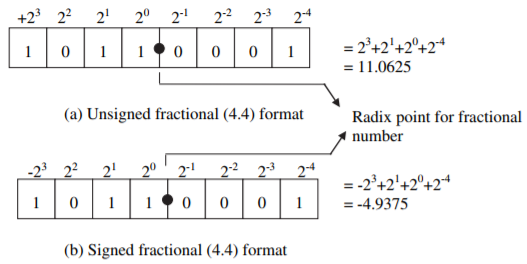
\includegraphics[width=0.6\linewidth]{graphics/1.png}
	\caption{Example of 8-bit binary data formats for a fractional number.}
	\label{fig:1}
\end{figure}

\begin{itemize}
	\item Dynamic Ranges and Precisions
	\begin{itemize}
		\item The maximum positive number in (1.15) format is $1 − 2^{−15} (= 0.999969482421875)$ (0x7FFF).
		\item The minimum negative number in (1.15) format is $−1$ (0x8000). 
		\item The 1.15 format has a \textbf{dynamic range} of $[+0.999969482421875$ to $−1]$
		\begin{itemize}
			\item Numbers exceeding this range cannot be represented in 1.15 format. 
		\end{itemize} 
		\item The smallest increment (or precision) within the (1.15) format is $2^{−15}$.
	\end{itemize}
\end{itemize}

\begin{figure} [H]
	\centering
	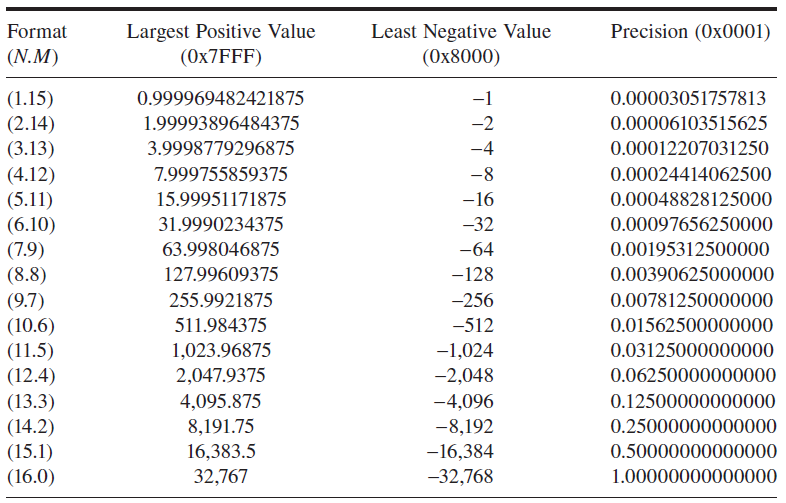
\includegraphics[width=\linewidth]{graphics/2.png}
	\caption{Dynamic ranges and precisions of 16-bit numbers using different formats.}
	\label{fig:2}
\end{figure}
\newpage
\begin{itemize}
	\item Scaling Factors
	\begin{itemize}
		\item A number in (N.M) format cannot be represented in the programs because most compilers and assemblers only recognize numbers in integer or (16.0) format. 
		\begin{itemize}
			\item Convert the fractional number in (N.M) format into its integer equivalent.
			\item Its radix point must be accounted for by the programmers.
			\begin{itemize}
				\item To convert a number $0.6$ in (1.15) format to its integer representation,
				multiply it by $2^{15}$ (or $32\,768$) and round the product to its nearest integer to
				become $19\,661$ (0x4CCD).
			\end{itemize}
		\end{itemize}
	\end{itemize}
\end{itemize}

\noindent\newline In Table \ref{fig:2} all 16 possible (N.M) formats for 16-bit numbers. Different formats give different dynamic ranges and precisions. There is a trade-off between the dynamic range and precision.
 \begin{itemize}
 	\item As the dynamic range increases, precision becomes	coarser.
 \end{itemize}
 


\begin{figure} [H]
	\centering
	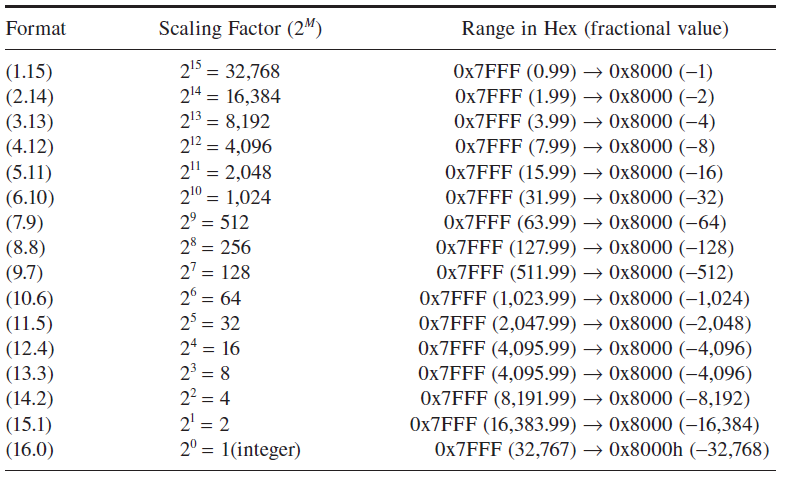
\includegraphics[width=\linewidth]{graphics/8.png}
	\caption{Scaling factors and dynamic ranges for 16-bit numbers using different formats.}
	\label{fig:8}
\end{figure}

\subsection{Conversion between different number formats}
\subsubsection{Fixed-Point Data Types}
The Blackfin C compiler supports eight scalar data types and two fractional data types.

\begin{figure} [H]
	\centering
	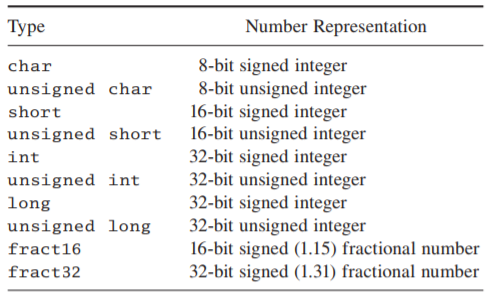
\includegraphics[width=0.8\linewidth]{graphics/3.png}
	\caption{Fixed-Point Data Types.}
	\label{fig:3}
\end{figure}

\subsection{(Blackfin) DSP Architecture}
\begin{itemize}
	\item Von Neumann architecture uses a single memory to hold both data and instructions.
	\item The Harvard architecture uses separate memories 
	for data and instructions, providing higher speed.
	\item The Super Harvard Architecture improves upon Harvard design by adding an instruction cache and a dedicated I/O controller.
\end{itemize}

\subsection{Choice of processor}
\begin{itemize}
	\item DSP
	\begin{itemize}
		\item Harvard memory architecture (optimized for the operational needs of digital signal processing).
		\item Handle real time processing, architecture is specially designed to fetch multiple data at the same time.
		\item Can handle floating numbers directly in the data flow path.
		\item Calculations are usually carried out by fixed point arithmetic process in order to speed them up.
	\end{itemize}
	\item Microcontroller
	\item General‐purpose CPU
	\begin{itemize}
		\item Most general-purpose CPU can also execute DSP algorithms, but dedicated DSPs usually have better power efficiency.
	\end{itemize}
	\item FPGA
	\item GPU
\end{itemize}

\subsection{Blackfin}
\begin{itemize}
	\item Blackfin is a \textit{MSA} Processor.
	\begin{itemize}
		\item MCU and DSP in same processor.
		\begin{itemize}
			\item Cheap and low power consumption.
		\end{itemize}
	\end{itemize}
	\item Architecture optimized for multimedia	processing (Audio and Video).
	\item Dataflow oriented tasks (DSP).
	\item Control flow oriented tasks (MCU).
	\item Good tools and compiler support.
\end{itemize}

\subsubsection{BF533 Overview}
\begin{itemize}
	\item 16-bit fixed-point processors	that are based on the MSA core.
	\item The processor targets power-sensitive applications (portable audio players, cell phones, digital cameras).
	\item Direct memory access (DMA) controller transfers data between external devices/memories and the internal memories without processor intervention.
	\begin{itemize}
		\item L1 cache memory for quick accessing of both data and instructions.
	\end{itemize}
	\item BF533 system peripherals:
	\begin{itemize}
		\item Parallel peripheral interface	(PPI)
		\item Serial peripheral interface (SPI)
		\item Serial ports (SPORTs)
		\item General-purpose timers
		\item Universal asynchronous receiver transmitter (UART)
		\item Real-time clock (RTC)
		\item Watchdog timer
		\item General-purpose input/output (I/O) ports
	\end{itemize}
\end{itemize}
\begin{figure} [H]
	\centering
	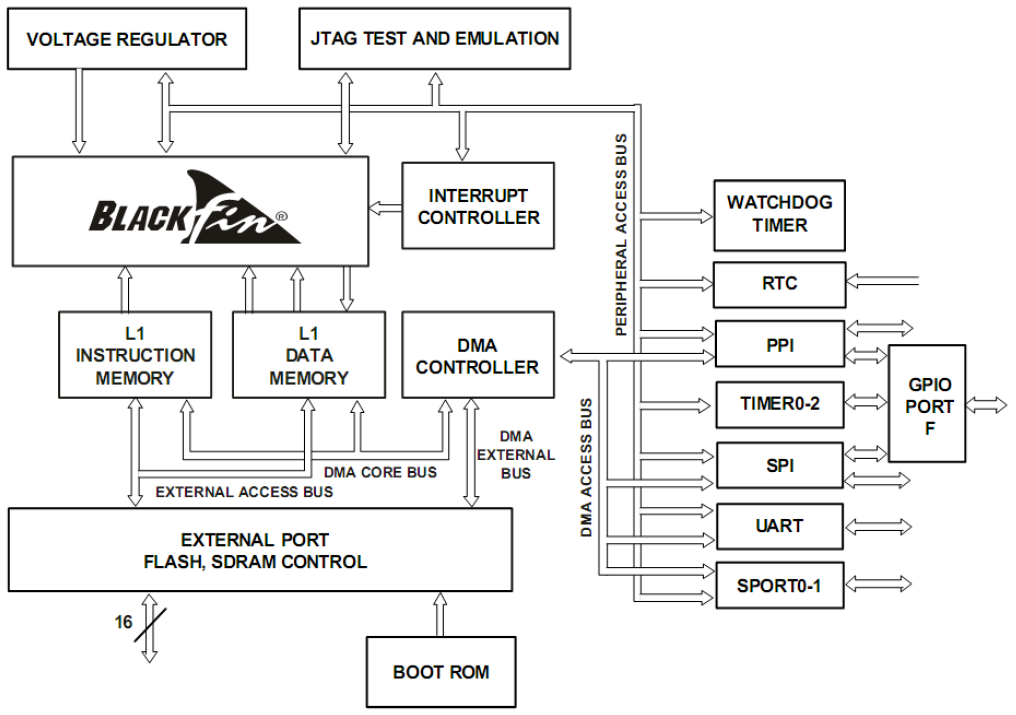
\includegraphics[width=0.85\linewidth]{graphics/6.png}
	\caption{BF533 Overview.}
	\label{fig:6}
\end{figure}

\subsubsection{Data Arithmetic Unit}
Computational units get data from data registers and perform fixed-point
operations. The data registers receive data from the data buses and transfer the data to the computational units for processing. Computational results
are moved to the data registers before transferring to the memory via data
buses.
\begin{itemize}
	\item Two 16-bit multipliers represented as $X_{16}$ in \ref{fig:7}.
	\item Two 40-bit accumulators (ACC0 and ACC1). 
	\begin{itemize}
		\item 16-bit lower-half (A0.L, A1.L)
		\item 16-bit upper-half (A0.H, A1.H)
		\item 8-bit extension (A0.X, A1.X)
	\end{itemize}
	\item Two 40-bit arithmetic logic units (ALUs) represented as $V_{40}$ in \ref{fig:7}.
	\item Four 8-bit video ALUs represented as $V_8$ in \ref{fig:7}.
	\item A 40-bit barrel shifter.
	\item Eight 32-bit data registers (R0 to R7) or 16 independent 16-bit registers (R0.L to R7.L and R0.H to R7.H).
\end{itemize}

\begin{figure} [H]
	\centering
	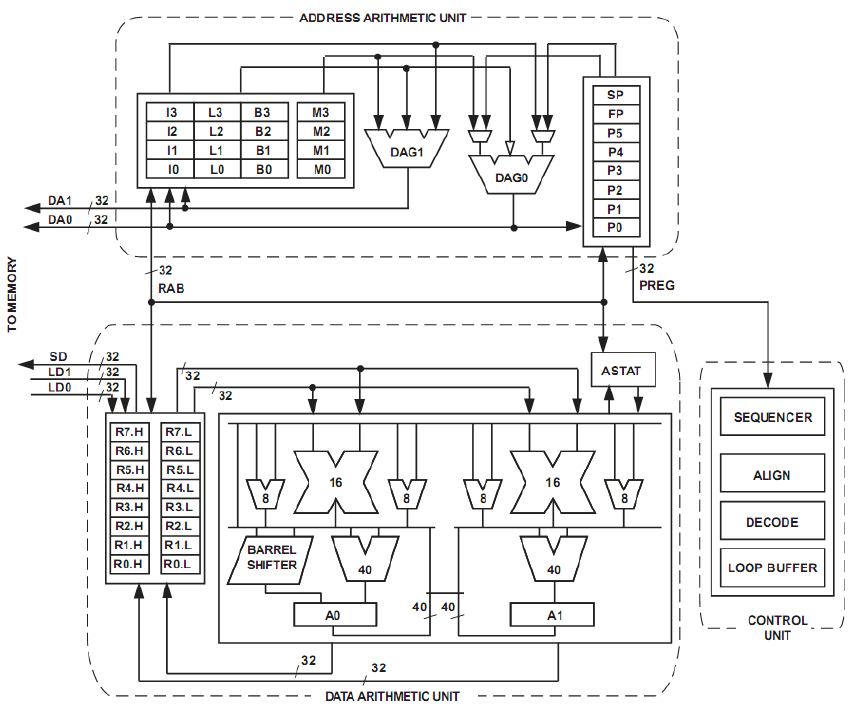
\includegraphics[width=\linewidth]{graphics/7.png}
	\caption{BF533 Core, Fixed-point processor.}
	\label{fig:7}
\end{figure}

\subsubsection{Arithmetic Operations}
\begin{itemize}
	\item Dual and single versions of add and sub
	\begin{itemize}
		\item Single 16-bit addition using three registers
		\begin{itemize}
			\item \mintinline{c}{R3.H = R1.L+R2.H (ns);}
			\begin{itemize}
				\item Saturation flag (s)
				\item No saturation flag (ns)
				\item End of instruction \textit{;}
			\end{itemize}
		\end{itemize}
		\item Dual 16-bit add/subtract using three registers
		\begin{itemize}
			\item \mintinline{c}{R3 = R1+|-R2;}
		\end{itemize}
		\item Quad 16-bit add/subtract using four registers
		\begin{itemize}
			\item \mintinline{c}{R3 = R1+|-R2, R4 = R1-|+R2;}
			\begin{itemize}
				\item Two operations can be operated on the same pair of 16-bit registers
				\item Separate two instructions operated at	same cycle \textit{;}
			\end{itemize}
		\end{itemize}
		\item Single 32-Bit Operations
		\begin{itemize}
			\item \mintinline{c}{R3 = R1+R2;}
		\end{itemize}
		\item Dual 32-Bit Operations
		\begin{itemize}
			\item \mintinline{c}{R3 = R1+R2, R4 = R1-R2}
		\end{itemize}
	\end{itemize}
\end{itemize}

\begin{figure} [H]
	\centering
	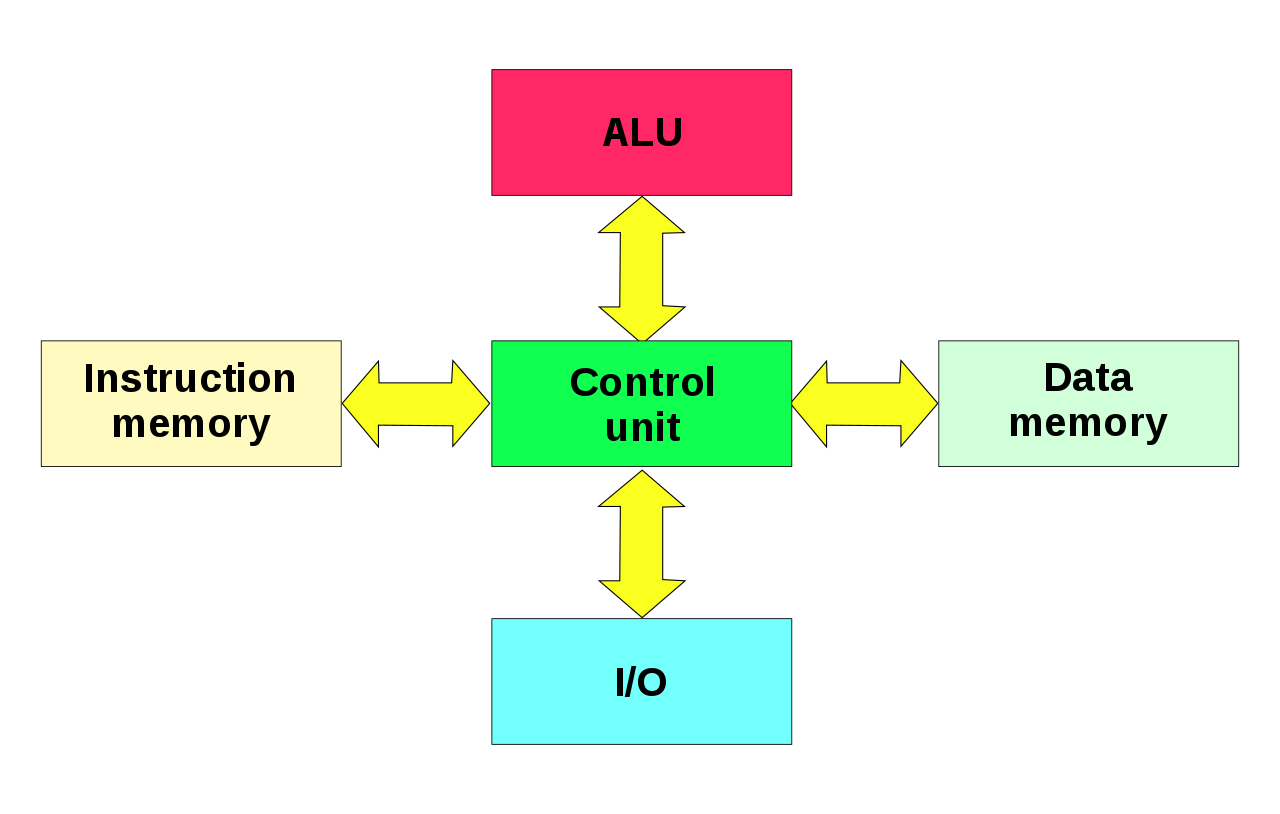
\includegraphics[width=\linewidth]{graphics/5.png}
	\caption{Arithmetic Modes and Options.}
	\label{fig:5}
\end{figure}

\begin{itemize}
	\item[] 
	\begin{itemize}
		\item Single 16-Bit Multiply Operations
		\begin{itemize}
			\item \mintinline{c}{R3 = R1.L*R2.H;}
		\end{itemize}
		\item Single 16-bit MAC using two registers and an accumulator
		\begin{itemize}
			\item \mintinline{c}{A0 += R1.L*R2.L;}
			\begin{itemize}
				\item Multiplies the contents of R1.L with R2.L, and the result is added to the value in the accumulator A0
			\end{itemize}
		\end{itemize}
		\item Dual 16-bit multiplications using two registers and two accumulators
		\begin{itemize}
			\item \mintinline{c}{A1 = R1.H*R2.H, A0 = R1.L*R2.L;}
			\begin{itemize}
				\item Two pairs of input are stored in registers R1 and R2
				\item Two 32-bit results are stored in the accumulators A0 and A1
			\end{itemize}
		\end{itemize}
		\item Dual 16-Bit Multiply Operations Using Two 32-Bit Registers
		\begin{itemize}
			\item \mintinline{c}{R0 = R2.H*R3.H, R1 = R2.L*R3.L}
			\begin{itemize}
				\item Dual 32-bit results are stored in R0 and R1
				\item Destination registers must be used in pairs as R0:R1, R2:R3, R4:R5, or R6:R7
			\end{itemize}
		\end{itemize}
	\end{itemize}
\end{itemize}


\begin{figure} [H]
	\centering
	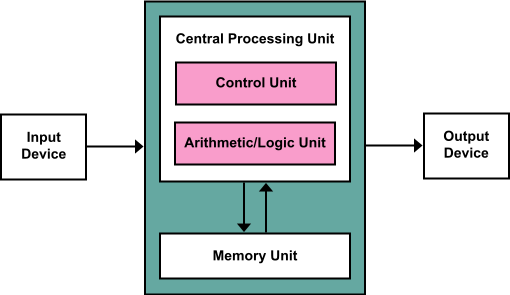
\includegraphics[width=\linewidth]{graphics/4.png}
	\caption{Multiplier Options.}
	\label{fig:4}
\end{figure}

\subsubsection{Address Arithmetic Unit}
The address arithmetic unit consists of the following hardware units:
\begin{itemize}
	\item Two data address generators (DAG0 and DAG1):
	\begin{itemize}
		\item Generate addresses for data moves to and from memory. The advantage of using two data address generators is to allow dual-data fetches in a single instruction.
	\end{itemize}
	\item Six 32-bit general-purpose address pointer registers (P0 to P5).
	\item One 32-bit frame pointer (FP) pointing to the current procedure's activation record.
	\item One 32-bit stack pointer (SP) pointing to the last location on the run time user stack.
	\item A set of 32-bit data address generator registers:
	\begin{itemize}
		\item Indexing registers, I0 to I3, contain the effective addresses.
		\item Modifying registers, M0 to M3, contain offset values for add/subtract with the index registers.
		\item Base address registers, B0 to B3, contain the starting addresses of the 	circular buffers.
		\item Length value registers, L0 to L3, contain the lengths (in byte unit) of the circular buffers.
	\end{itemize}
\end{itemize}

\subsubsection{Control Unit}
A program sequencer controls the instruction execution flow, which includes
instruction alignment and instruction decoding. The address generated by
the program sequencer is a 32-bit memory instruction address. A 32-bit
program counter (PC) is used to indicate the current instruction being
fetched.

\begin{figure} [H]
	\centering
	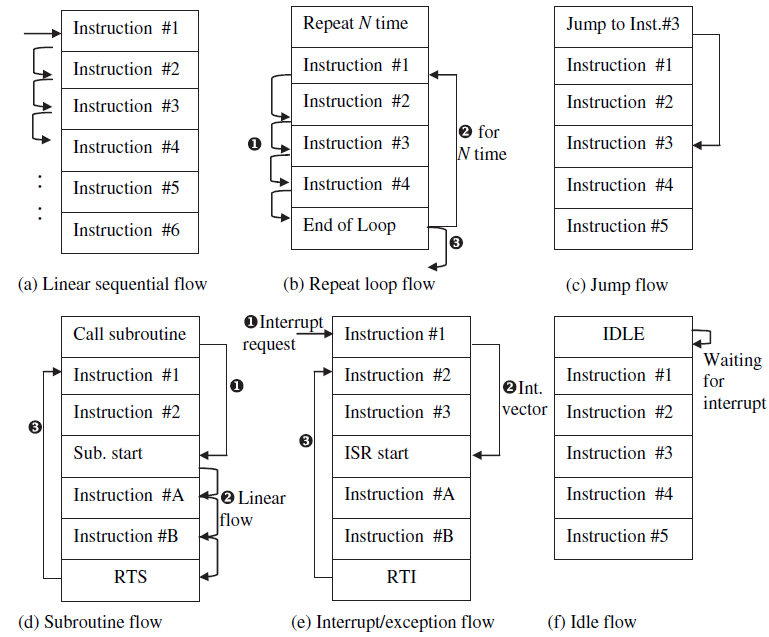
\includegraphics[width=\linewidth]{graphics/16.png}
	\caption{Different types of program flow.}
	\label{fig:16}
\end{figure}

The pipeline is used to maximize the distribution of workload among the processor's functional units, which results in efficient parallel processing among the processor's hardware. The Blackfin processor has a 10-stage instruction pipeline. 

\begin{figure} [H]
	\centering
	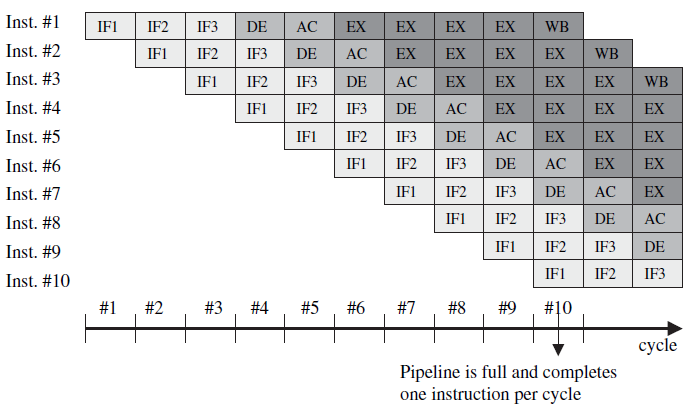
\includegraphics[width=\linewidth]{graphics/14.png}
	\caption{Ten pipeline stages of the Blackfin processor.}
	\label{fig:14}
\end{figure}

Each instruction can be executed in a single clock cycle when the pipeline
is full, giving a throughput of one instruction per clock cycle. However, any
nonsequential program flow (Fig. \ref{fig:16}) can potentially decrease the
processor's throughput.

\begin{figure} [H]
	\centering
	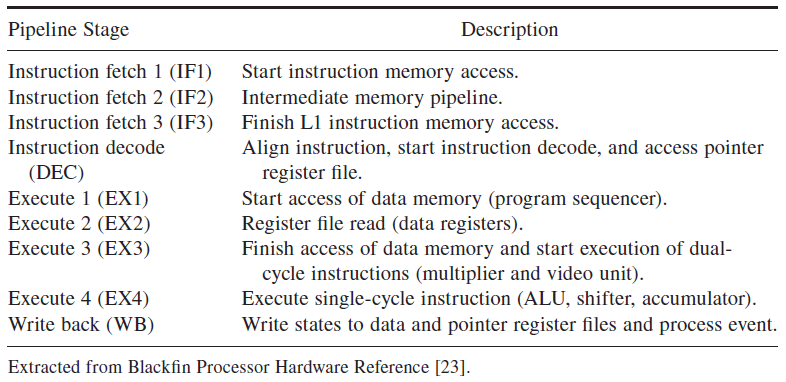
\includegraphics[width=\linewidth]{graphics/15.png}
	\caption{Stages of Instruction Pipeline.}
	\label{fig:15}
\end{figure}